\documentclass[
	12pt, % Default font size, values between 10pt-12pt are allowed
	%letterpaper, % Uncomment for US letter paper size
	%spanish, % Uncomment for Spanish
]{fphw}

% Template-specific packages
\usepackage{inputenc} % Required for inputting international characters
\usepackage[T1]{fontenc} % Output font encoding for international characters
\usepackage{mathpazo} % Use the Palatino font
%\usepackage{ctex}
\usepackage{graphicx,subfigure} % Required for including images
\usepackage{booktabs} % Required for better horizontal rules in tables
\usepackage{listings}
\usepackage{listings} % Required for insertion of code
\usepackage{fontspec}
\usepackage{enumerate} % To modify the enumerate environment
\usepackage{amsmath}
\usepackage{amssymb}
\usepackage{mathptmx}
\usepackage{bm}
%----------------------------------------------------------------------------------------
\setmainfont{Times New Roman}
%----------------------------------------------------------------------------------------
%----------------------------------------------------------------------------------------
%	ASSIGNMENT INFORMATION
%----------------------------------------------------------------------------------------

\title{Homework \#4} % Assignment title

\author{NAME SID} % Student name and ID

\date{November 12, , 2020} % Due date

\institute{SOUTHERN UNIVERSITY\\OF SCIENCE AND TECHNOLOGY} % Institute or school name

\class{Modern Control and Estimation (MEE 5106)} % Course or class name

\professor{Prof. Wei Zhang} % Professor or teacher in charge of the assignment

%----------------------------------------------------------------------------------------

\setlength{\abovecaptionskip}{-0.1cm}
\setlength{\belowcaptionskip}{0cm}   %调整图片标题与下文距离
\begin{document}

\maketitle % Output the assignment title, created automatically using the information in the custom commands above

%----------------------------------------------------------------------------------------
%	ASSIGNMENT CONTENT
%----------------------------------------------------------------------------------------

\section*{Question 1}
\begin{problem}
	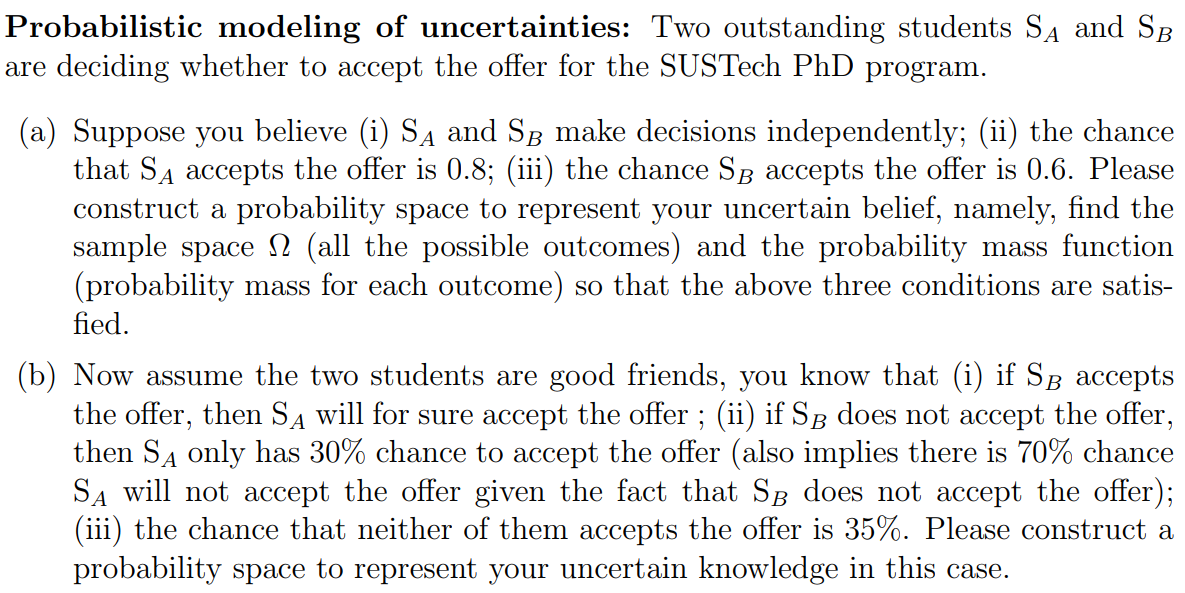
\includegraphics[width=440pt]{img/q1.png}
\end{problem}

%------------------------------------------------

\subsection*{Answer}
\begin{enumerate}[(\itshape a\normalfont)]
    \item From the Question 1(a), we have the $P(S_A)=0.8$ and $P(S_B)=0.6$, the $S_A$ and $S_B$ make decisions independently means that $P(S_AS_B)=P(S_A)P(S_B)$, So we have all the possible outcomes are $S_AS_B, \bar{S_A}S_B, S_A\bar{S_B}, \bar{S_A}\bar{S_B}$, the notation $\bar{S_A}$ means $S_A$ does not accept the offer. And the probability mass function of those outcomes are :
    \begin{equation}\nonumber
        \begin{array}{c}
        P(S_AS_B)=P(S_A)P(S_B)=0.48 \\
        P(S_A\bar{S_B})=P(S_A)P(\bar{S_B})=0.32\\
        P(\bar{S_A}S_B)=P(\bar{S_A})P(S_B)=0.12\\
        P(\bar{S_A}\bar{S_B})=P(\bar{S_A})P(\bar{S_B})=0.08
    \end{array}   
    \end{equation}
    
    \item From the Question 1(b), we can get the probability of $P(S_A|S_B)=1$, $P(S_A|\bar{S_B})=0.3$ and $P(\bar{S_A}\bar{S_B})=0.35$. From the \textbf{Conditional probability's} definition
    \begin{equation}\nonumber
        P(A|B) = \frac{P(AB)}{P(B)}
    \end{equation}
\end{enumerate}
%----------------------------------------------------------------------------------------
\clearpage
\section*{Question 2}
\begin{problem}
	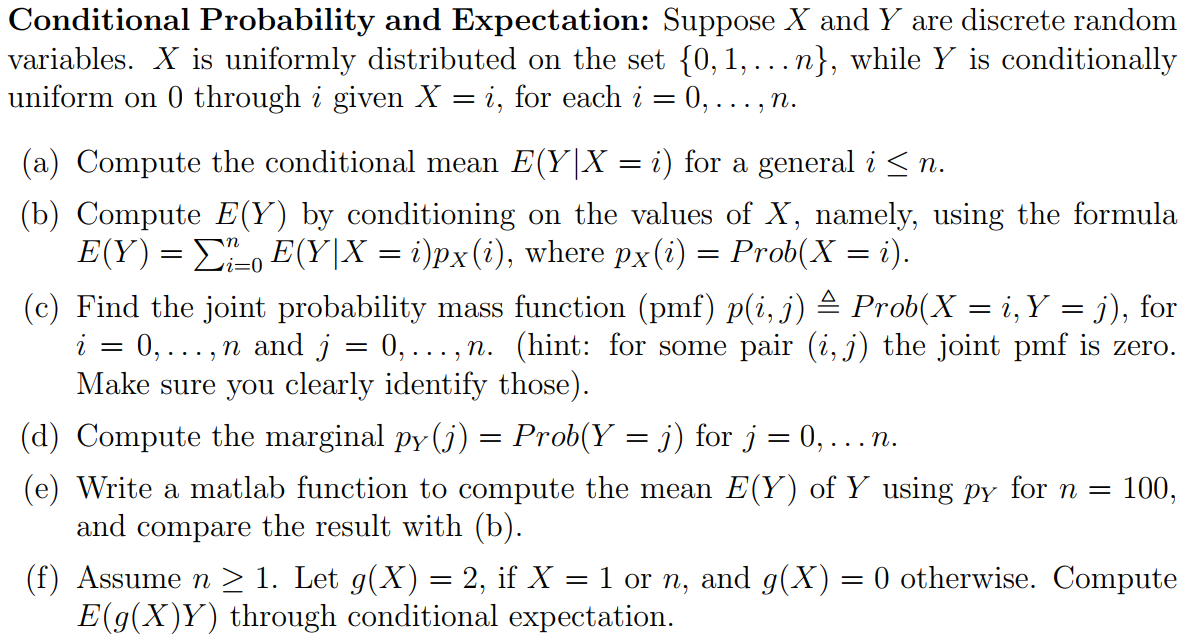
\includegraphics[width=440pt]{img/q2.png}
\end{problem}

%------------------------------------------------

\subsection*{Answer}
\begin{enumerate}[(\itshape a\normalfont)] % Sub-questions styled as italic letters
	\item ssssIdentify the author of Equation below and briefly describe it in Latin.
	\begin{equation}\label{eq:bayes}
		P(A|B) = \frac{P(B|A)P(A)}{P(B)}
	\end{equation}
\end{enumerate}

%----------------------------------------------------------------------------------------
\clearpage
\section*{Question 3}
\begin{problem}
    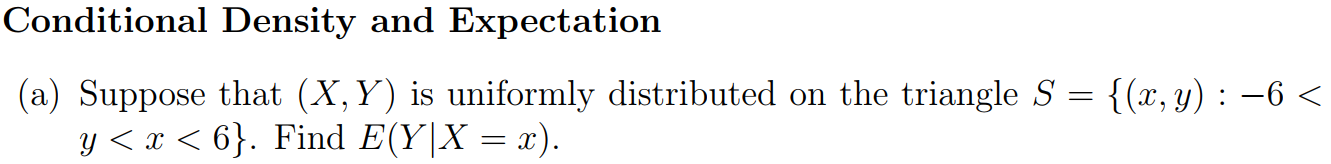
\includegraphics[width=440pt]{img/q3_1.png}\\
    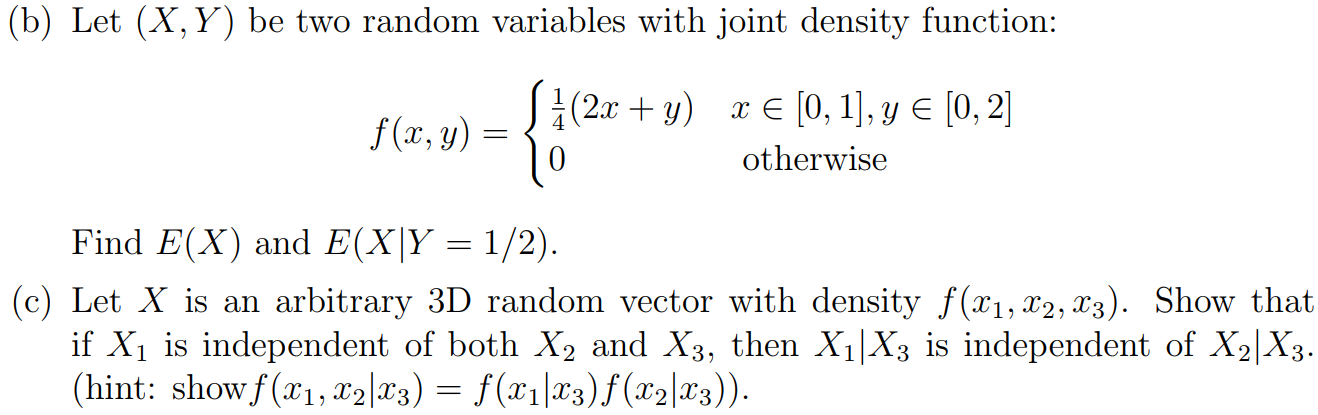
\includegraphics[width=440pt]{img/q3_2.png}
\end{problem}

%------------------------------------------------

\subsection*{Answer} 
\begin{enumerate}[(\itshape a\normalfont)]
    \item sss 
\end{enumerate}

%----------------------------------------------------------------------------------------
\clearpage
\section*{Question 4}

\begin{problem}
    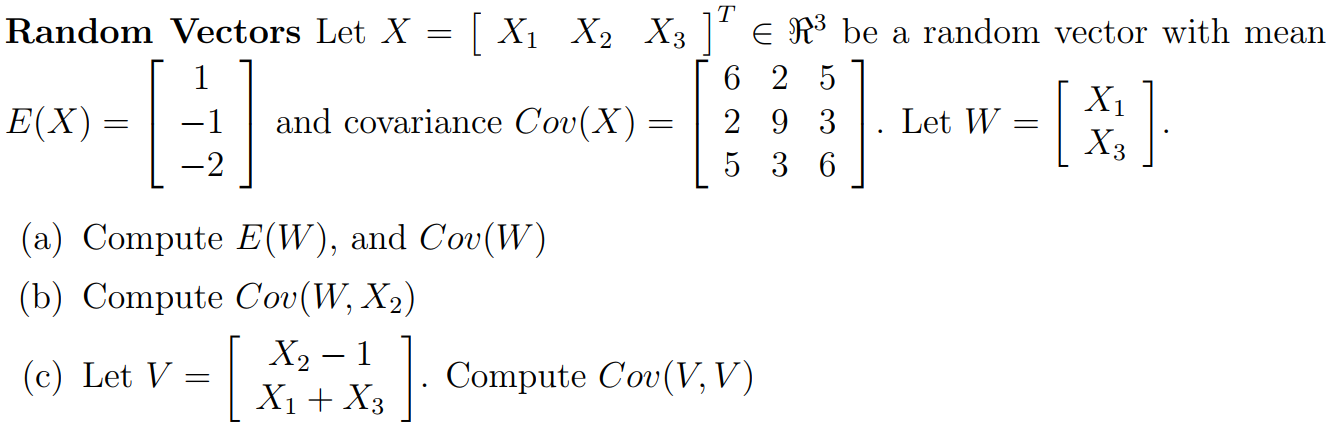
\includegraphics[width=440pt]{img/q4.png}
\end{problem}

%------------------------------------------------

\subsection*{Answer}
\begin{enumerate}[(\itshape a\normalfont)]
    \item sss 
\end{enumerate}
	The table below shows the nutritional consistencies of two sausage types. Explain their relative differences given what you know about daily adult nutritional recommendations.
	
	\bigskip
    
	\begin{center}
		\begin{tabular}{l l l}
			\toprule
			\textit{Per 50g} & Pork & Soy \\
			\midrule
			Energy & 760kJ & 538kJ\\
			Protein & 7.0g & 9.3g\\
			Carbohydrate & 0.0g & 4.9g\\
			Fat & 16.8g & 9.1g\\
			Sodium & 0.4g & 0.4g\\
			Fibre & 0.0g & 1.4g\\
			\bottomrule
		\end{tabular}
	\end{center}
	
	\medskip


%----------------------------------------------------------------------------------------
\clearpage
\section*{Question 5}
\begin{problem}
	\lstinputlisting[
		caption=Luftballons Perl Script, % Caption above the listing
		label=lst:luftballons, % Label for referencing this listing
		language=Perl, % Use Perl functions/syntax highlighting
		frame=single, % Frame around the code listing
		showstringspaces=false, % Don't put marks in string spaces
		numbers=left, % Line numbers on left
		numberstyle=\tiny, % Line numbers styling
	]{code/code.m}
	
	\begin{enumerate}
		\item How many luftballons will be output by the Listing above?
		\item Identify the regular expression in Listing  and explain how it relates to the anti-war sentiments found in the rest of the script.
	\end{enumerate}

\end{problem}

%------------------------------------------------

\subsection*{Answer}

\begin{enumerate}
	\item 99 luftballons.
	\item Lorem ipsum dolor sit amet, consectetur adipiscing elit. Praesent porttitor arcu luctus, imperdiet urna iaculis, mattis eros. Pellentesque iaculis odio vel nisl ullamcorper, nec faucibus ipsum molestie. Sed dictum nisl non aliquet porttitor. Etiam vulputate arcu dignissim, finibus sem et, viverra nisl. Aenean luctus congue massa, ut laoreet metus ornare in. Nunc fermentum nisi imperdiet lectus tincidunt vestibulum at ac elit. Nulla mattis nisl eu malesuada suscipit.
\end{enumerate}

%----------------------------------------------------------------------------------------

\end{document}
